\chapter{Computer System with Project Work}

\newpage

\section{M1}
\subsection{CPU}
The central processing unit (CPU) is the electronic circuitry within a
computer that carries out the instructions of a computer program by
performing the basic arithmetic, logical, control and input/output (I/O)
operations specified by the instructions.

\subsection{Register}
A processor register is a quickly accessible location available to a
computer’s central processing unit (CPU). Registers usually consist of
a small amount of fast storage. A CPU only has a small number of
registers.

\subsection{Memory}
Memory refers to the computer hardware integrated circuits that store
information for immediate use in a computer; it is synonymous with the
term “primary storage”. The memory is much slower than the CPU
register but much larger in size.
Sources

\subsection{CPU context}
At any point in time, the values of all
the registers in the CPU defines the
CPU context. Sometimes CPU state

\subsection{Memory allocation}
\begin{figure}[h]
    \vspace{10mm}
    \centering
    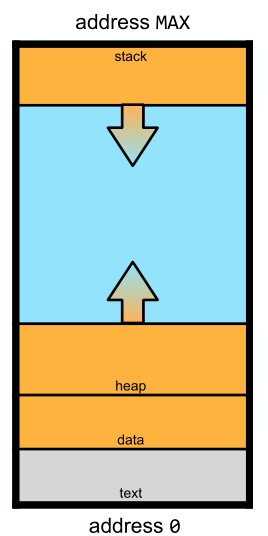
\includegraphics[width=5cm, height=10cm]{image/memory-allocation.png}
    \caption{memory-allocation}
\end{figure}

\subsection{Kernal}
The kernel is a computer program
that is the core of a computer’s
operating system, with complete
control over everything in the
system.

\subsection{Multiprogramming}
\begin{figure}[h]
    \vspace{10mm}
    \centering
    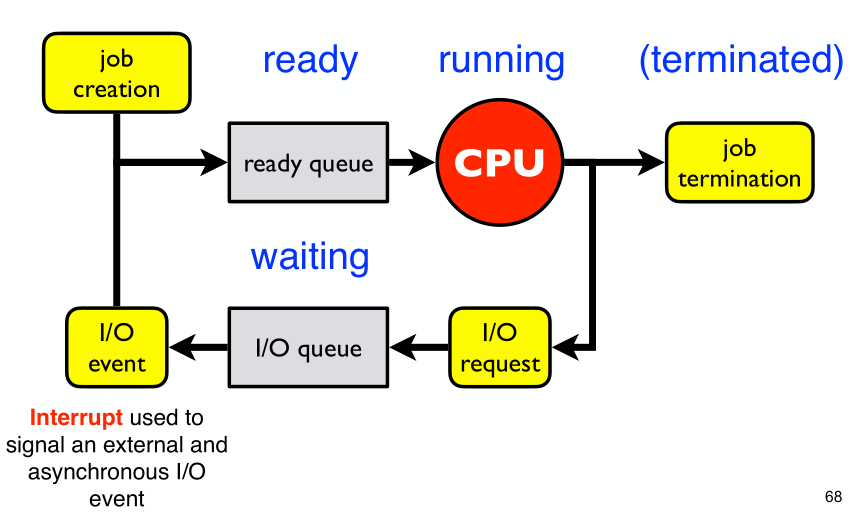
\includegraphics[width=14cm, height=10cm]{image/multiprogramming.png}
    \caption{multiprogramming}
\end{figure}

\section{M2}
\subsection{Network communication}
\begin{figure}[h]
    \vspace{10mm}
    \centering
    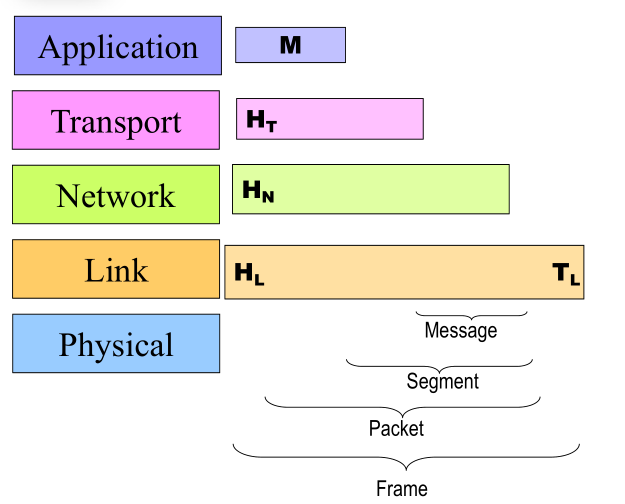
\includegraphics[width=14cm, height=10cm]{image/layering.png}
    \caption{layering}
\end{figure}

\begin{itemize}
\item TCP for a reliable byte stream service
\item UDP for an unreliable message forwarding service
\item Four different delivery models: uni/broad/multi/any-cast
\item The client/server model is common in application design
\item Sockets API can be used for network programming
  \begin{itemize}
  \item A socket is a communication handle abstraction
  \item Properties of a socket can be set through socket options
  \end{itemize}
\end{itemize}

\subsection{Prossesses}
\begin{itemize}
\item Zombie: A terminated process is said to be a zombie or defunct until the
\item Orphan: An orphan process is a process whose parent process has terminated, though it remains running itself.
\item Signals: are a limited form of inter-process communication used in
\item File discriptor: The kernel keeps a table with information about a process’s open file descriptors.
\item Pipes: An (anonymous) pipe is a simplex FIFO communication channel that may be used for
\end{itemize}

\section{M3}
\begin{itemize}
\item DNS är ett distribuerat system av servrar
\item ARP mappar IP-address till länklageraddress
\item En IP-address har två delar för att identifiera nätve
\end{itemize}

\begin{figure}[h]
    \vspace{10mm}
    \centering
    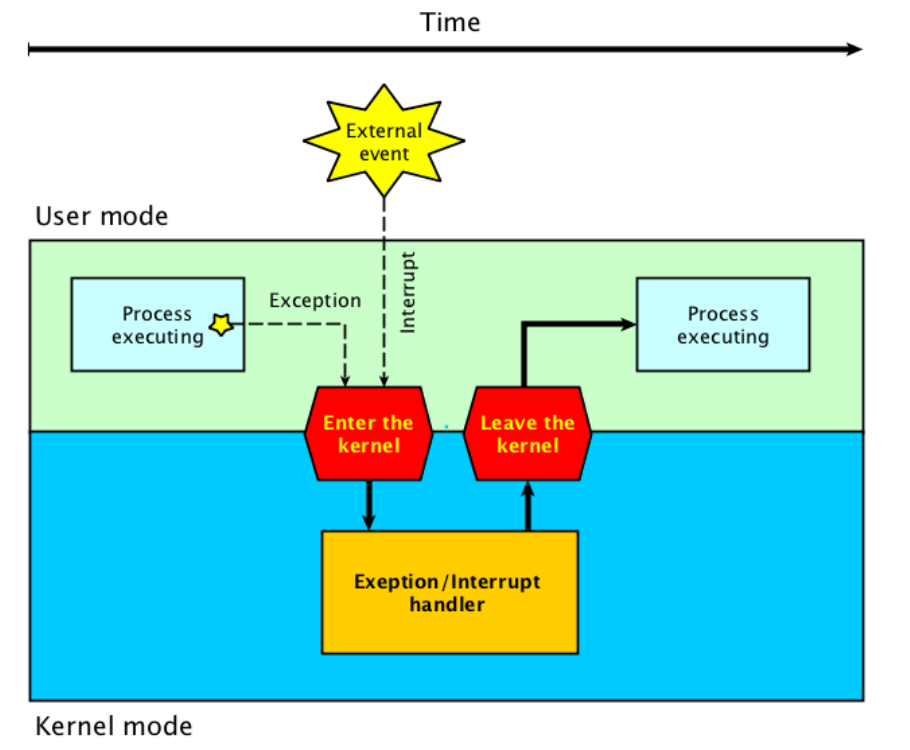
\includegraphics[width=14cm, height=10cm]{image/user-kernal-mode.png}
    \caption{user-kernal-mode}
\end{figure}

\subsection{Dispatcher}
Another component that is involved in the
CPU-scheduling function is the dispatcher,
which is the module that gives control of the
CPU to the process selected by the short-
term scheduler. It receives control in kernel
mode as the result of an interrupt or system
call.  \newline

The CPU scheduler selects one process from among the
processes in memory that are READY to execute. The
scheduler dispatcher then gives the selected process control

\subsection{PSB}
The process control block (PCB) is a data
structure in the operating system kernel
containing the information needed to
manage a particular process. \newline

The Long-term scheduler (LTS) (aka job
scheduler) decides whether a new process should
be brought into the ready queue in main memory
or delayed. \newline

The medium-term scheduler (MTS) temporarily remove processes from
main memory and places them in secondary storage and vice versa,
which is commonly referred to as "swapping in" and "swapping out".

\subsection{IO bound/CPU bound}
An I/O-bound process spends
more time doing I/O than
computations and is characterised \newline

An CPU-bound process spends
more time doing computations and
is characterised by few very long

Interactive processes interact constantly with their human
users.  \newline

Batch processes do not interact with human users. \newline

Real-time processes have very strong scheduling
requirements.

\subsection{Schedular algorithems}
The first come, first served (commonly called FIFO ‒ first
in, first out) process scheduling algorithm is the simplest
process scheduling algorithm. Processes are executed on
the CPU in the same order they arrive to the ready queue. \newline


Shortest Job First (SJF) scheduling assigns the process
estimated to complete fastest, i.e, the process with
shortest CPU burst, to the CPU as soon as CPU time is avalible. \newline

An extension of SJF where the currently running process is P
preempted if the CPU burst of a process A arriving to the ready
queue is shorted than the remaining CPU burst of the currently
running process. \newline

A priority number (integer) is associated with each process.
The CPU is allocated to the process with the highest priority
(smallest integer = highest priority). \newline

Round Robin (RR) is a scheduling algorithm where time slices
are assigned to each process in equal portions and in circular
order. \newline

A multi-level queue scheduling algorithm is used in scenarios where
the processes can be classified into groups based on properties like
process type, CPU time, IO access, memory size, etc. \newline

In computer science, starvation is a problem encountered in
multitasking where a process is perpetually denied necessary
resources. Without those resources, the process can never finish its
task. \newline

Ageing is used to ensure that jobs with lower
priority will eventually complete their
execution.

\section{M4}
\subsection{Concurrency}
The ability of different parts or units of a
program, algorithm, or problem to be executed
out-of-order or in partial order, without affecting

\subsection{Parallelism}
In parallel systems, two tasks
are actually performed
simultaneously.
Parallelism is when tasks

\subsection{Client-Server modle}
A distributed application structure that partitions
tasks or workloads between the providers of a
resource or service, called servers, and service
requesters, called clients.

\subsection{Threads}
A thread of execution is the smallest sequence of instructions
that can be managed independently by a scheduler, which is
typically a part of the operating system.

\subsubsection{Atomic}
In concurrent programming, an operation (or
set of operations) is atomic if it appears to the
rest of the system to occur at once without
being interrupted.

\subsubsection{Race condition}
A race condition or race hazard is the
behaviour of an electronic, software or other
system where the output is dependent on the
sequence or timing of other uncontrollable
events.

\subsubsection{Data race}
A data race occurs when two instructions from
different threads access the same memory location

\subsection{Locks}
In general, any solution to the
critical section problem requires a
tool/abstraction - a lock.

\subsection{Spinlock}
A spinlock is a lock where a task
simply waits in a loop ("spins")
repeatedly checking until the lock
becomes avalible.

\subsection{TestAndSet}
The TestAndSet instruction
atomically first sets the value at the
target address to True and return the
old value stored at the target address.

\subsection{Swap}
The Swap instruction atomically
swaps the content of two memory

\subsection{Bounded waiting}
A bound must exist on how many
times a task has to wait in order to
enter a critical section.

\subsection{Semaphores}
The hardware solutions to the critical section
problem using Swap and TestAndSet are
complicated for programmers to use directly.


\subsection{Mutex lock}
Many locking libraries provides a special
mutex lock which can only be used to
provide mutual exclusion to critical sections.

\subsection{Deadlock}
In concurrent computing, a deadlock is
a state in which each member of a
group is waiting for some other member
to take action, such as sending a
message or more commonly releasing a lock.

\subsection{Mutual exclusion}
A chopstick can only be held by one
philosopher at the time.
Updating the amount of rice must be atomic.

\subsection{Deadlock prevention}
Preventing deadlocks by constraining how requests for
resources can be made in the system and how they are
handled (system design).

\subsection{Deadlock avoidance}
The system dynamically considers every request and
decides whether it is safe to grant it at this point,

\subsection{Clock Synchronization}
\begin{itemize}
\item External synchronization
\item Internal synchronization
\item Hard in an asynchronous system
\end{itemize}

\subsection{Mutual exclusion}
\begin{itemize}
\item Critical section
\item Need for coordination:
\item Evaluation criteria for different solutions
\end{itemize}


\subsection{Desired properties of Transactions}
\begin{itemize}
\item Atomicity
\item Consistency
\item Isolation
\item Durability
\end{itemize}

\subsection{WiFi}
\begin{itemize}
\item Several standards, from 2Mbit/s to 100’s of Mbit/s
  \begin{itemize}
    \item Using multiple channels for higher speeds
  \end{itemize}
\item Range: in general 20-100m, depending on the environment
\item Can be used in ad hoc or infrastructure mode
  \begin{itemize}
    \item Ad Hoc: like a wireless Ethernet
    \item Infrastructure: a coordinating base station
  \end{itemize}
\item Networks identified with SSID:s
  \begin{itemize}
    \item Used to scramble signal somewhat
  \end{itemize}
\item Encryption with WEP (bad), WPA(better), WPA2 (best)
\end{itemize}

\subsection{Bluetooth}
 \begin{itemize}
\item Several different versions
  \begin{itemize}
    \item Different transmission power (and hence ranges)
  \end{itemize}
\item Different profiles for different applications
\item Frequency hopping 1600 times/s in ISM band
\item Peer to peer or piconet networks
\item Max 7 simultaneous connections
\end{itemize}

\subsection{ISM-band}
\begin{figure}[h]
    \vspace{10mm}
    \centering
    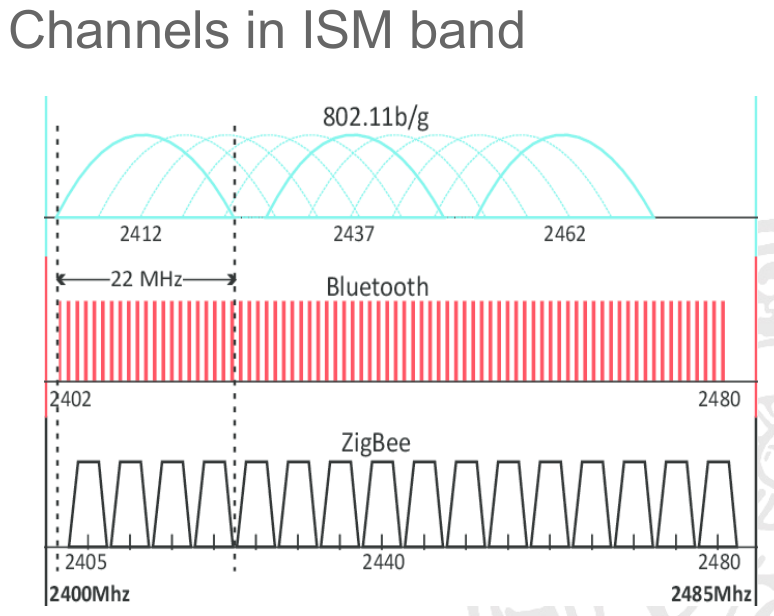
\includegraphics[width=12cm, height=10cm]{image/ISM-band.png}
    \caption{ISM-band}
\end{figure}

\subsection{Properties of a medium}
\begin{itemize}
\item Bandwidth B
  \begin{itemize}
    \item Frequency range for signals transmitted in medium
  \end{itemize}
\item Signal/noise ratio S/N, SNR
  \begin{itemize}
    \item Frequency range for signals transmitted in
    \item Signal level / noise level
    \item Measured at the receiver
    \item Can be approximated with Maxwell’s equations
  \end{itemize}
\item Capacity C=B log2 (1+S/N)
\end{itemize}

\subsection{Sampling}
Bandwidth B Hz is sampled at 2*B Hz

\subsection{Multithreading models}
\begin{figure}[h]
    \vspace{10mm}
    \centering
    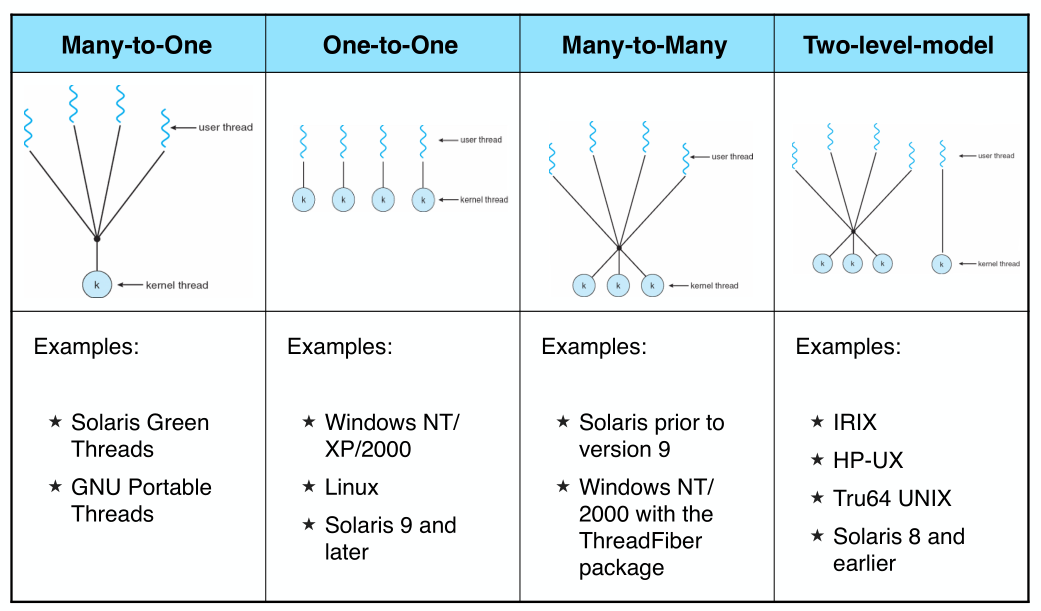
\includegraphics[width=16cm, height=10cm]{image/Multithreading-models.png}
    \caption{Multithreading-models}
\end{figure}

\subsection{Bounded buffer}
A bounded buffer lets multiple producers and multiple
consumers share a single buffer. Producers write data to

\subsection{Priority inversion}
A higher priority task is “preempted” by a lower priority one.

\section{M5}
\subsection{Single contiguous}
Single contiguous allocation is the simplest
memory management technique. All the
computer's memory, usually with the
exception of a small portion reserved for
the operating system, is available to the
single application.

\subsection{Swapping}
A process can be swapped temporarily
out of memory to a backing store, and
then brought back into memory for continued execution.

\subsection{Memory resident}
Certain programs, can be marked as being
memory resident, which means that the operating
system is not permitted to swap them out to a
storage device; they will always remain in
memory.

\subsection{Partitioned allocation}
Partitioned allocation divides primary memory into multiple memory
partitions, usually contiguous areas memory.

\subsection{Logical address space}
A logical address is the address at which
a memory cell appears to reside from the perspective of an
executing application program.

\subsection{Address binding}
Address binding is the process of mapping
the program's logical (or virtual addresses)
to corresponding physical memory
addresses.

\subsection{Memory management unit (MMU)}
 The MMU is a computer hardware unit having
all memory references passed through itself,
primarily performing the translation of logical
memory addresses to physical addresses.

\subsection{Fragmentation}
Fragmentation is a phenomenon in which
storage space is used inefficiently, reducing
capacity and often performance.

\subsection{Compaction}
Move all processes to one end of the address
space producing one large hole at the other
end of the address space.

\subsection{Memory protection}
Memory protection between
processes implemented by
associating a valid bit with each
entry in the per process page table.

\subsection{Shared pages}
Paging makes it possible for
processes to share parts of their
memory space with each other.

\subsection{Translation lookaside buffer}
A translation lookaside buffer (TLB) is a
memory cache that is used to reduce the time
taken to access a user memory location.
The TLB stores the recent translations of virtual memory to physical memory.

\subsection{Operating System}
Controls the hardware and
coordinates its use among the
various application programs for various users.

\subsection{Access methods}
Data can be accessed in different patterns. These
patterns can be divided into two main categories:
Sequential access,
Random access (aka direct access)

\subsection{RAM}
The main memory aka primary memory
is a form of Random Access Memory (RAM).

\subsection{Volatile memory}
Volatile memory, in contrast to non-volatile memory, is computer
memory that requires power to maintain the stored
information; it retains its contents while powered on but when
the power is interrupted, the stored data is quickly lost.

\subsection{Persistent data storage}
In computer science, persistence refers to the
characteristic of state that outlives the process
that created it.

\subsection{The file}
A file is a named collection of related
information that is recorded on
secondary storage.

\subsection{Block data storage}
A file is made up of fixed length logical recordes (blocks)

\subsection{File control block}
A File Control Block (FCB) is a file
system structure in which the state of an
open file is maintained.

\subsection{Directory}
 A directory is a file system cataloging
structure which contains references to
other computer files, and possibly other directories.

\subsection{Contiguous allocation}
Each file occupies a set of contiguous blocks on the disk.

\subsection{Linked allocation}
Each file is a linked list of disk blocks: blocks may be
scattered anywhere on the disk.

\subsection{Indexed allocation}
Indexed allocation brings all pointers together into an index

\subsection{FAT}
File Allocation Table (FAT) is a computer file
system architecture and a family of industry-
standard file systems utilizing it. The FAT file
system is a legacy file system which is simple and robust.

\subsection{iNode}
In Unix-style file systems the file control
block is called iNode.
The inode is a data structure that
describes a filesystem object such as
a file or a directory.

\subsection{Directory}
 A directory is a file system cataloging
structure which contains references to
other computer files, and possibly other
directories.

\subsection{M6}
\subsection{Classic historical ciphers}
Caesar cipher (monoalphabetic),
Vigenere cipher (polyalphabetic).

\subsection{Modern cryptography}
If a lot of smart people for a long time have failed to solve a specific problem,
it is unlikely that a solution will appear soon. \newline

\begin{itemize}
\item Encryption method is well-known
\item Secret guarded by a n-bit key
  \begin{itemize}
    \item Encryption and decryption in $O(n)$ time
    \item Key guessing in $O(2^n)$ time
  \end{itemize}
\item Key management is crucial
\item CIA triad represent desirable properties
  \begin{itemize}
  \item Confidentiality
  \item Integrity
  \item Availability
  \end{itemize}
\end{itemize}

\subsection{Public key exchange}
\begin{center}
\begin{tabular}{ c c }
 Alice & Bob \\
 Create secret key $S_A$ & Create secret key $S_B$ \\
 Compute $T_A=g^{S_A} \: mod \: p$ & Compute $T_B=g^{S_B} \: mod \: p$ \\
 Send $T_A$ to Bob & Send $T_B$ to Alice \\
 Compute $K_1=T_B^{S_A} \: mod \: p$ & Compute $K_2=T_A^{S_B} \: mod \: p$ \\
\end{tabular}
\end{center}

\begin{figure}[h]
    \vspace{10mm}
    \centering
    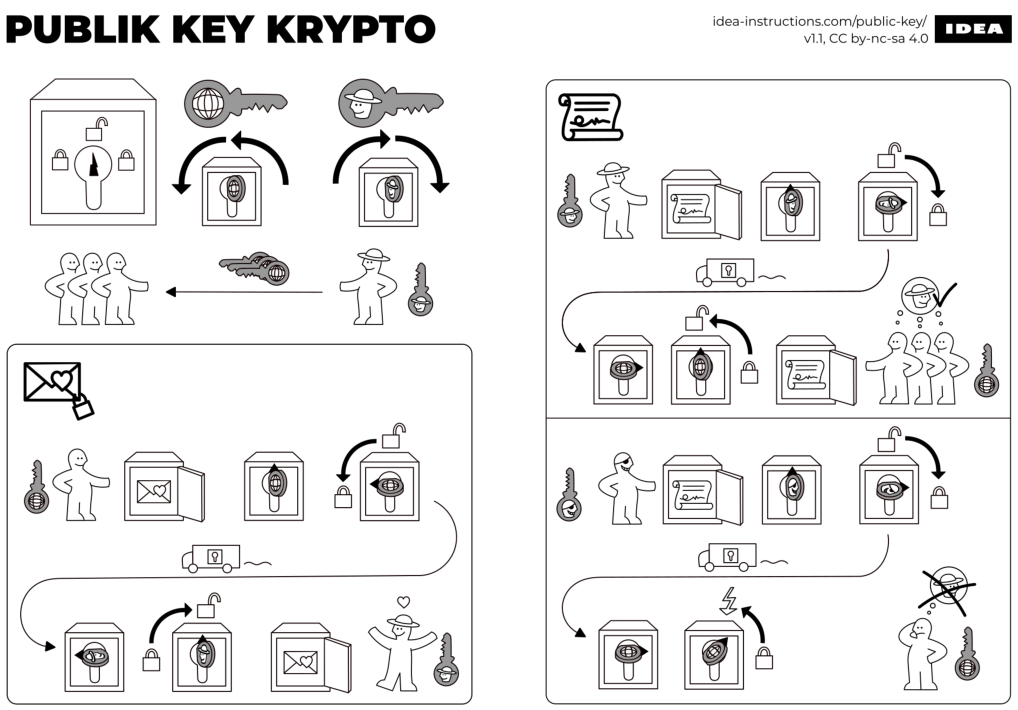
\includegraphics[width=16cm, height=10cm]{image/publik-key-krypto.png}
    \caption{publik-key-krypto}
\end{figure}

\subsection{Certification Authority (CA)}
Issues digital certificates: Digitally signed with the private key of the CA,
Authorize a public key.

\subsection{Chain of trust}
\begin{figure}[h]
    \vspace{10mm}
    \centering
    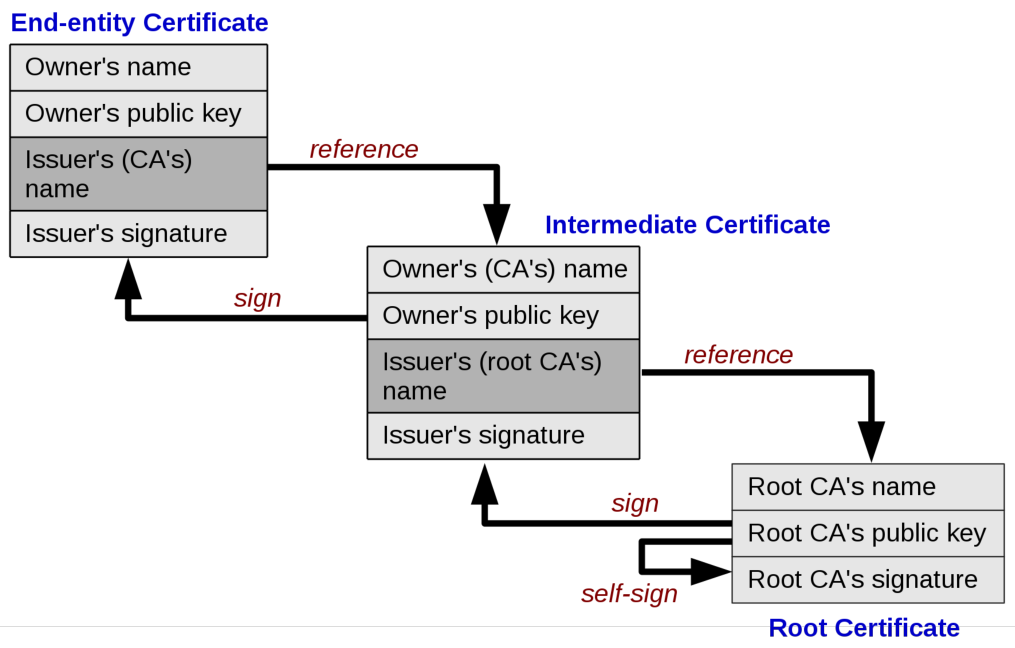
\includegraphics[width=16cm, height=10cm]{image/chain-of-trust.png}
    \caption{chain-of-trust}
\end{figure}

\subsection{Self-issued certificates}
Some sites present self-issued certificates: A little lite designing your own drivers license.

\subsection{Usage of modern cryptography}
\begin{itemize}
\item Symmetric cryptography in encrypted sessions
  \begin{itemize}
    \item public-key cryptography not fast enough
  \end{itemize}
\item Asymmetric cryptography in certain situations
  \begin{itemize}
  \item To establish a symmetric key
  \item Digital signatures and verification
  \end{itemize}
\item Cryptographic hashing for verification of authentic data
\end{itemize}

\subsection{Man-in-middle attack}
the attacker secretly relays and possibly alters the communications between two parties who believe that they are directly communicating with each other
\subsection{Chosen-plaintext attack}
presumes that the attacker can obtain the ciphertexts for arbitrary plaintexts. The goal of the attack is to gain information that reduces the security of the encryption scheme
\subsection{Side-channel attack}
any attack based on information gained from the implementation of a computer system, rather than weaknesses in the implemented algorithm itself
Timing information, power consumption, electromagnetic leaks or even sound can provide an extra source of information, which can be exploited.
\subsection{Replay attack}
valid data transmission is maliciously or fraudulently repeated or delayed. This is carried out either by the originator or by an adversary who intercepts the data and re-transmits it, possibly as part of a spoofing attack by IP packet substitution. This is one of the lower-tier versions of a man-in-the-middle attack. Replay attacks are usually passive in nature.

\subsection{Security in the Internet stack}
\begin{itemize}
\item Application layer: DNSSEC
\item Transport layer: SSL/TLS
\item Network layer: IPsec
\item Link layer: WEP/WPA, MAC filtering, ...
\end{itemize}

\subsection{Firewall}
\begin{figure}[h]
    \vspace{10mm}
    \centering
    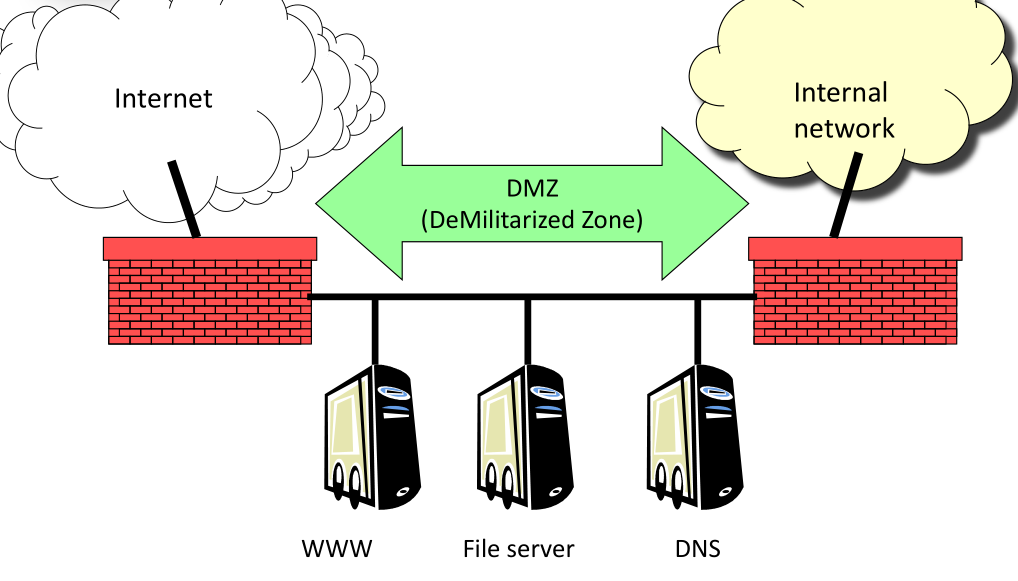
\includegraphics[width=16cm, height=10cm]{image/firewall.png}
    \caption{firewall}
\end{figure}
